%\documentclass[acmsmall]{acmart}
\documentclass[sigconf]{acmart}

\usepackage{graphicx}
\graphicspath{images/}

%%
%% \BibTeX command to typeset BibTeX logo in the docs
\AtBeginDocument{%
  \providecommand\BibTeX{{%
    \normalfont B\kern-0.5em{\scshape i\kern-0.25em b}\kern-0.8em\TeX}}}

%% Rights management information.  This information is sent to you
%% when you complete the rights form.  These commands have SAMPLE
%% values in them; it is your responsibility as an author to replace
%% the commands and values with those provided to you when you
%% complete the rights form.
\setcopyright{acmcopyright}
\copyrightyear{2020}
\acmYear{2020}
\acmDOI{10.1145/1122445.1122456}

%%
%% These commands are for a JOURNAL article.
\acmJournal{JACM}
\acmVolume{37}
\acmNumber{4}
\acmArticle{111}
\acmMonth{8}

\begin{document}

%%TW: Titles suggestions depending on result/discussion chapter?:

%\title{Leveraging healthcare data wrangling and data analytics in a pandemic era}

%\title{The power of data warehousing and prediction models for uncovering multinational spread of infectious diseases}

%\title{Towards data wrangling and analytics for preventive actions on new waves of Covid-19 pandemic}


\title{Towards Solving the World}
%29TH ACM INTERNATIONAL CONFERENCE ON INFORMATION AND KNOWLEDGE MANAGEMENT \\ Data and information acquisition and pre-processing \\ or Integration and aggregation}

%% VJ: THIS NEEDS TO BE COMMENTED OUT AS IT IS DOUBLE-BLIND REVIEW PROCESS
%% \author{Andreas Francois Vermeulen}
%% \email{afv@st-andrews.ac.uk}
%% \orcid{0000-0003-2225-6851}
%% \authornotemark[1]

%% \author{Juliana K\"uster Filipe Bowles}
%% \email{jkfb@st-andrews.ac.uk}

%% \author{Thais Webber}
%% \email{tcwds@st-andrews.ac.uk}

%% \author{Juan Mendoza Santana}
%% \email{jjm20@st-andrews.ac.uk}

%% \affiliation{%
%%   \institution{University of St Andrews}
%%   \streetaddress{Jack Cole Building, North Haugh}
%%   \city{St Andrews}
%%   \state{Scotland, United Kingdom}
%%   \postcode{KY16 9SX}
%% }

%% \author{Vladimir Janjic}
%% \email{VJanjic001@dundee.ac.uk}

%% \affiliation{%
%%   \institution{University of Dundee}
%%   \streetaddress{Nethergate}
%%   \city{Dundee}
%%   \state{Scotland, United Kingdom}
%%   \postcode{DD1 4HN}
%% }


%% \author{Euan Blackledge}
%% \email{euan.blackledge@soprasteria.com}

%% \affiliation{%
%%   \institution{Sopra Steria}
%%   \streetaddress{30 Queensferry Rd}
%%   \city{Edinburgh}
%%   \state{Scotland, United Kingdom}
%%   \postcode{EH4 2HS}
%% }

%% \renewcommand{\shortauthors}{Vermeulen A.F, Bowles J.K.F, Vladimir V, Blackledge E, Webber T and Santana J.M}
%% END OF AUTOR LIST

\begin{abstract}
  The Rapid Information Factory enables SERUMS project to create an effective and efficient processing solution to generate a hyper-scale data processing factory.

This rapid information factory assists the data wrangling of the Covid-19 data as supplied by the various healthcare in counties. This is the core deliverable of the SERUMS project.

This paper shows that the lack of an processing methodology similar to the rapid information factory has during the Covid-19 pandemic causes damaging delays and misinformation that hampered effective and efficient deployment of resources to most needed areas.

Our research shows that .... 
\end{abstract}


\keywords{datasets, data processing, data lake, data warehouse, data wrangling, covid-19}
%%TW: data warehouse design, data wrangling, data analytics, disease surveillance, covid-19


%%
%% This command processes the author and affiliation and title
%% information and builds the first part of the formatted document.
\maketitle

\url{https://cikm2020.org/call-for-papers-full-and-short-research-papers/}

\section{Introduction}

%TW notes:
%find possible focus/title?? "Leveraging healthcare data warehousing and data analytics in a pandemic era" 
%%for predictions of pandemics and infectious diseases spread?
%%for the surveillance of possible new waves of pandemic Covid-19?
%%SERUMS data analytics unveiling new waves of Covid-19 pandemic? for multinational preparedness plans?

{\color{red}{VJ: What problem are we solving here? We talked today about the problem of having inaccurate data about the number of infections, which then hampers the appropriate planning of where to deploy resources etc. We can use this as a motivational story in introduction, to point out that lack of proper sharing of information between health centres can literally cost lives. The question then is how we are solving this problem? How does RIF help with this? Do we have/can we get any results that show this? If we go by this route, I propose the following organisation of the paper:
    \begin{itemize}
    \item Section 1 - Introduction: a paragraph about general COVID information, a paragraph about inaccurate information about infections/deaths, probably with some nice diagram which shows the number of reported cases is not really following any 'normal' trajectory and that we have points where nubmer of infections/deaths inexplainably drops (e.g. over weekends). Here we should also explain why this is due to lack of information sharing rather than the practice used in reporting deaths (which we cannot really influence). Then a paragraph about RIF and the SERUMS infrastructure we are using and how it helps with the problems outlined above. Then a list of research contributions.
    \item Section 2 - Rapid Information Factory and SERUMS project: Here we describe what SERUMS is about and also describe RIF in some detail. This could be our background section, if RIF was described elsewhere in research publications.
    \item Section 3 - Impact of Problems with Sharing Medical Information in Time of COVID-19: Here we elaborate what the problem is. This is a more detailed description of the problem, probably with more graphs.
    \item Section 4 - Our Solution: This is where we describe how RIF is used to help with the problems identified in introduction and expanded on in Section 3.
    \item Section 5 - Experimental Results.
    \item Section 6 - Related Work.
    \item Section 7 - Conclusions and Future Work.
    \end{itemize}

    I don't really see where the model to predict the number of infections would fit into and this doesn't sound as a particular research novelty (unless we develop a better model than the existing ones, which would probably be impossible to prove). But if we go for some other angle, that could change things.
}}

The Serums Project (Securing Medical Data in Smart Patient-Centric Healthcare Systems)\footnote{\url{https://www.serums-h2020.org/}} is an European Union Horizon 2020 research project that supports security and privacy of future-generation healthcare systems, placing the patients at the centre of future healthcare provision, enhancing their personal care and maximising the quality of treatment citizens receive. 

The Coronavirus disease (COVID-19) shows how the currently lack of integration and aggregation of healthcare data across the world.

Our hyper-scaling data crawler methodology enables processing factory that can process the data in the healthcare.

\begin{itemize}
    \item Data and information acquisition and processing (e.g., data crawling, data quality, data privacy, mitigating biases, and data wrangling)
    \item Integration and aggregation (e.g., semantic processing, data provenance, data linkage, data fusion, knowledge graphs, data warehousing, privacy and security, modelling, information credibility)
\end{itemize}

The solution enables the integration of healthcare data and knowledge for the next generation to support the sustainability, transparency and fairness of the worldwide view of the combined the healthcare.

\section{Rapid Information Factory (RIF)}

The SERUMS project use the \emph{Rapid Information Factory} to enforce an effective and efficient data wrangling processing for the various data formats.

The Rapid Information Factory is a processing methodology that uses design concepts adopted out of the Production Economics' Manufacturing Production methodologies by adopting the three basic manufacturing concepts into data processing:

make to stock (MTS)
predictable demand

Antonio Arreola-risa and Gregory A. DeCroix in \cite{Arreola-Risa1998} explain how effective balance between make-to-order (MTO) versus make-to-stock (MTS) for producing multiple heterogeneous products can be achieved in a shared manufacturing facility. The same principal translated via transferable learning into a data processing context. 

\begin{itemize}
    \item make to order (MTO) predictable demand for a product and then built upfront.
    \item make-to-stock (MTS) allows customers to order products built to their specifications
    \item make to assemble (MTA) hybrid of MTS and MTA in that companies stock basic parts based on demand predictions, but do not assemble them until customers place their order. 
\end{itemize}

\section{Rapid Information Engine}

We used a Dask scheduler with 8 x Dual (64 core/128 threads per socket) AMD AEPYC 7552 Processors with 64 GB Ram and four Seagate IronWolf 110 Series 1.92TB SSD Drives clusters. This enabled us to have 1024 core/2048 treads 512 GB RAM and 60 TB disk space for data lake.

The software used is Ubuntu with Charmed Kubernetes and MAAS (Metal-as-a-Service). The Dask clusters are then created on top of Kubernetes to ensure a flexible processing ecosystem.

The workcells in the factory always setup as part of the programming blueprint.




\section{Data Lake Zones}

The healthcare research is persisted in a data lake.

\section{Work-space Zone}

The work space zone is the temporary or trenchant storage space in the data lake to assist the data processing data crawlers to store data results and then share it with other down-stream processing data crawlers.

\section{Raw Zone}

The raw zone is data lake zone that stores the source system data in its original source format. It does not hold any structure meta-data.

The data crawlers that perform the data acquisition from the Covid-19 data sources stores their results into this zone for downstream processing.

%%TW: data crawlers operate in the work-space and in the raw zone then? not clear since both section mention the storage of results


We used the following data sources:
\begin{itemize}
    \item Time
    We use a fix range start on 2019-12-01 until 2020-12-01 ensure we capture any of the data sources.
    \item Person
    We used a GDPR \cite{EU2017} compliance methods of creating the right distribution of persons without compromising the individual person rights.
    %%data sets have general statistics of population and individuals behaviour.. no? or we are talking about serumers records (actual patient records/info)?
    \item Object
    As to the objects used in the data set we have only limited the objects to three objects called Covid-19, hospital bed and ICU Bed. This purely because we did not track or process the other objects like hospital beds, masks etc. %%not clear
    \item Location
    The location was one of the major part of our research as we wanted to understand how location and factors about that location impacted the Covid-19 pandemics evolution across the globe. Our location is stored as a latitude and longitude to the tenth decimal using the latitude and longitude projection called the World Geodetic System (WGS) 1984 coordinate system.
    \item Event
    The event is the second major part of our research as it tracks every event that happens within the Covid-19 ecosystem.
    The following events are tracked:
    \begin{itemize}
        \item Patient Zero
        \item Patient exposed to virus
        \item Has Covid-19 virus
        \item Person infects other person
        \item Person in hospital bed
        \item Person in ICU bed
        \item Person died
        \item Person recovers
    \end{itemize}
\end{itemize}

\subsection{Active Data Sources}

We used the following data sources for our paper:

\begin{itemize}
    \item Static List of the European countries (Valid Dec 2020)
    \item Dynamic update from Novel Coronavirus (COVID-19) Cases, provided by JHU CSSE 
\end{itemize}

%%%%%%%%%%%%%%%%%%%%%%%%%%%%%%%%%%%%%%%%%%%%%%%%%%%%%%%%%%%%%%%%%%%%%%%%

\section{Structured Zone}

The structured zone storage the results of the data crawlers that processes data via the retrieve super-step data crawlers.

%% Hold data types, Field name made the same pre-possessing of data


%%%%%%%%%%%%%%%%%%%%%%%%%%%%%%%%%%%%%%%%%%%%%%%%%%%%%%%%%%%%%%%%%%%%%%%%
\section{Curated Zone}
%% Private publish - Next deliverable - Built offline
%% When you ready publish
This zone holds the end results of the data and information aggregation.

The Curated zone storage the results of the data crawlers that processes data via the assess, transform, process, organise and report super-steps' data crawlers.

This is the zone that holds the Covid-19 data vault, data warehouse and data marts

%% data vault 2.0 format - Time-Person-Object-Location-Event Hub
%% data vault => data warehouse (everything) => data marts (UK, USA)

The use of a Rapid Information Factory can enable a hyper-personalised customer experience by analysing the data at a global level and at the lowest data-leave level by simply running the correct queries. That is the advantage of having a hyper-scale-able factory with hyper-personalised data processing.

The processing in this zone is not impacting the active customers of the Covid-19 insights published as the processing is done offline in a pre-processing cluster that has the appropriate processing capability.

Once the data is turned into business insights it is bulk copied (published) to the consumer and analytic zones. This ensures minimum disruption of the consumer and analytic adhoc processing.

%%%%%%%%%%%%%%%%%%%%%%%%%%%%%%%%%%%%%%%%%%%%%%%%%%%%%%%%%%%%%%%%%%%%%%%%
\section{Consumer Zone}
%% Online to customer => publish <= hospital at data

%% data marts as-is from Curated zone (copy) - business intelligence

The consumer zone is the storage accessed by the front-office customers when running the pre-processed business intelligence and pre-trained data science models. The core deliverable for our Covid-19 processing is our graphs showing how the lack of timely data updates and retrospective changes to already published facts are showing an incomplete and incorrect view of the true business insights.


%%%%%%%%%%%%%%%%%%%%%%%%%%%%%%%%%%%%%%%%%%%%%%%%%%%%%%%%%%%%%%%%%%%%%%%%
\section{Analytic Zone}

%% data warehouse - Data science plus data analysis (bulk big queries)

The analytic zone is the storage zone for any data required by further down-stream processing and becomes the source data for several other data science investigations. We will not include those as they are future research we will publish at later date.
\section{Data Crawler}

The data crawler is the smallest data processing unit within the data factory. The data crawler is evolved using a blue print of the R-A-P-T-O-R pipeline and bills-of-material consisting of code snippets and then spawn with an unique identity. Our data processing data crawlers is built to perform a single purpose and then made extinct once it completes the specific task.

\begin{figure}{!h}
    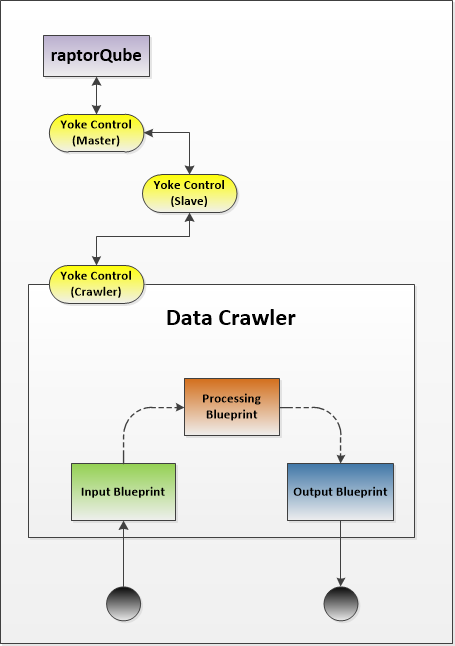
\includegraphics[width=3cm]{images/DataCrawler.png}
    \caption{Basic Data Crawler Blueprint.} \label{fig:datacrawler}
\end{figure}

The basic template for the data crawler (fig. \ref{fig:datacrawler}) is:

\begin{itemize}
    \item raptorQube - Core autonomous processing engine that controls the complete solution.
    \item Yoke Control (Master) - Master control yoke of data factory.
    \item Yoke Control (Slave) - Slave control yoke of data factory.
    \item Data Crawler - the crawler is the work cell for the processing.
    The crawler is evolve and spawn to perform a singular task in the processing workflow pipeline.
    The crawler consists of following to enable its dynamic processing.
    \begin{itemize}
        \item Yoke Control (Crawler)
        \item Input Blueprint
        \item Processing Blueprint
        \item Output Blueprint
    \end{itemize}
\end{itemize}

The factory supports the following types of crawlers:
\begin{itemize}
    \item Rapid Assimilator - crawler builds the ecosystem for each factory.
    \item Scout - crawler scouts for new or changed data entities in the ecosystem for each factory.
    \item Explorer - crawler explores any entities found by scout.
    \item Builder - crawler builds the processing pipeline for the R-A-P-T-O-R engine in the ecosystem for each factory.
    \item Monitor - crawler monitors the ecosystem to collect information about each factory's ecosystem.
\end{itemize}


\section{Data Vault}
Our chosen storage format for the data is a data vault~\cite{Linstedt2015}. It allows for new sources of data to be added without the need for a complex redesign of the existing data structures. Additionally, it places an emphasis on data lineage and provenance, ensuring accountability is maintained for any processes taking place on the platform. 

Both the flexibility to accommodate change, and the emphasis on recording the data's journey, will be important factors as more data sets are combined from health services around the world. The ability to consume massively different styles, schemas, and formats of source data, bring them into a single format, and ensure accountability for this transformation is vital as part of any platform wishing to be both powerful, and transparent.

The structure of a data vault relies on three component table types. These are:
\begin{itemize}
    \item Hubs - carries the business keys of the data set
    \item Links - joins the hubs together
    \item Satellites - joined to the hubs and carries the descriptive data in small tables, each one containing only very closely related data
\end{itemize}

\begin{figure}[H]
    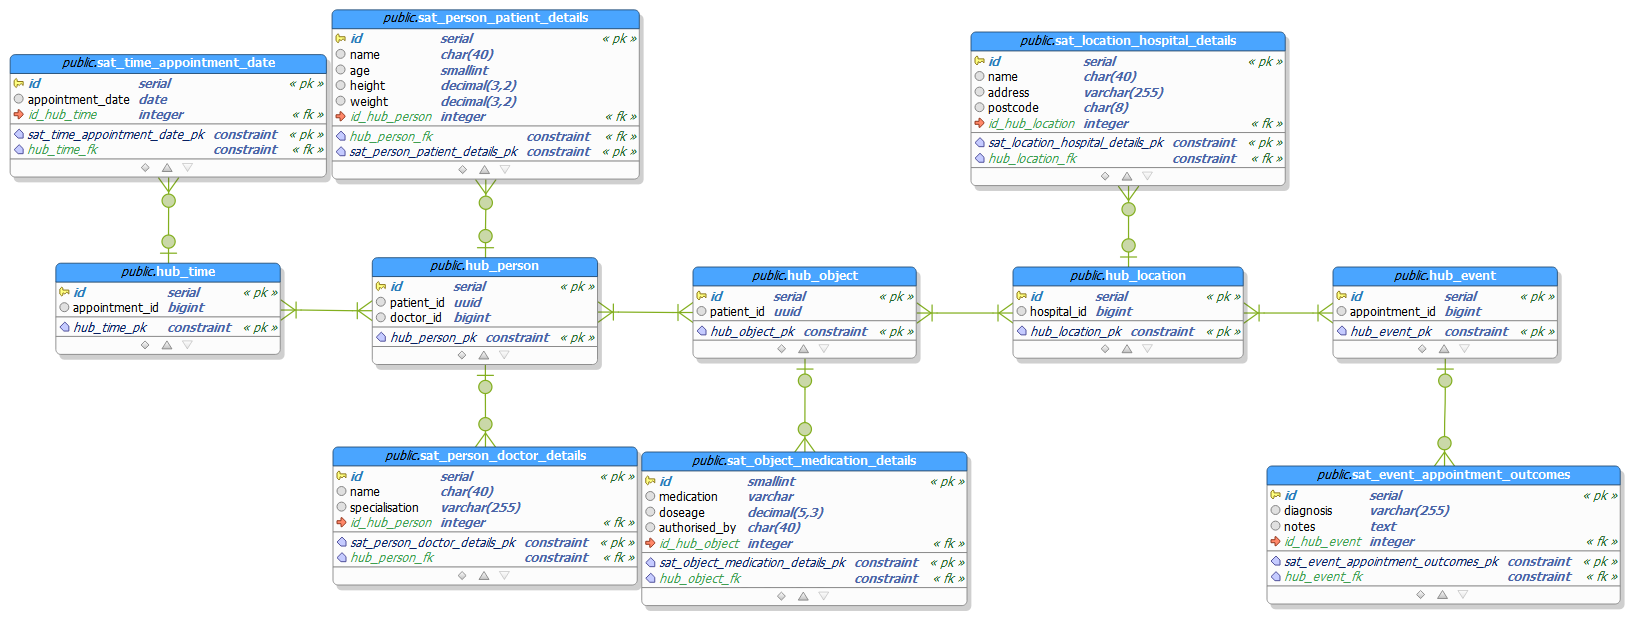
\includegraphics[width=12cm]{images/tpole_plus_sats.png}
    \caption{An example data vault. Hubs form the backbone with Satellites carrying the descriptive details} 
    \label{fig:tpole_sats}
\end{figure}

The Hubs form the backbone of the data vault structure and are used to categorise the data. For our purposes, we have chosen Time, Person, Object, Location, and Event (TPOLE). With these five categories, we are able to classify any of the incoming data. 

With a category assigned to each new piece of data, it is then evaluated as to whether it is closely related enough to the contents of any existing Satellite, under the same category. If it is closely enough related, it will be added to that Satellite, otherwise it will be placed in a new one. This process can be repeated at any stage, whenever a new data source is identified without the destruction of any of the existing data within the data vault.

The trade-off for this flexibility is the need to understand the incoming data. Currently this is a manual process in the Serums \cite{janjic2019serums} project, however plans are in place to introduce elements of machine learning in order to speed this up.

For our Covid-19 project we used a simple rules engine that forms a weak AI to match the data into the T-P-O-L-E categories that then directly mapped into one of the hubs of the data vault.

\section{Covid-19 Issues}

Bill Gates states in his research "Responding to Covid-19 — A Once-in-a-Century Pandemic?" that the virus has ability to kill healthy adults as well as elderly people with recognise health complications. The current accepted fatality risk ratio around 0.01. Simple terms 1 in 100 infected is at risk. The virus transmission rate or reproduction number \cite{medicalnews001} is between 2.0 to 3.0. The serial interval (time between one person developing the symptoms of a condition and a second person becoming infected and developing symptoms) is < 4 days with a silent transmission rate \cite{medicalnews001} is 0.1. 
The asymptomatic carriers rate (contracted virus but display no symptoms) \cite{medicalnews001} is 0.01 and 0.03.

The incubation time concludes that the median for developing symptoms is 5.1 days, and 97.5\% of those developing symptoms do so within 11.5 days.

%% https://www.healthline.com/health/r-nought-reproduction-number#rsubsubvalues
%% R0

%% Model & Simulation??
%% here some material on SIR model
%% https://triplebyte.com/blog/modeling-infectious-diseases
%%idea: find recent mathematical models, and parameters requirements - to analyse SERUMS capability on delivering analytics

Requirements from data processing solution.
%% ?


Gates \cite{Gates2018} predicted that world needs to accelerate work on treatments and vaccines for Covid-19 

Jay van Wyk \cite{Wyk2015} states global hyper-connectivity and increased system integration generates various benefits like (worldwide growth in incomes, education, innovation, and technology). All of these growth is driven by our ability to share data and processes. The downside is that the same rapid globalisation now has repercussions of local events regularly cascading over national borders and the fallout of financial meltdowns and environmental disasters immediately affects everyone. This increasingly dynamics and turbo-charged globalisation has now destabilise our societies by carrying a virus across the globe through the same optimised transport systems that was driving our global growth till weeks ago.

%% TW: disease surveillance must appear in the paper title maybe

disease surveillance, including a case database that is instantly accessible to relevant organisations, and rules requiring countries to share information.

Gates in 1999 \cite{Gates1999}  that business develop a  “digital nervous system” that feeds metrics on the state and trends in the business. Our research has shown that a similar concept using our rapid information factory to drive a self-healing data factory can process healthcare data like the data on Covid-19.

\section{The Raw Data}

The raw base data from Johns Hopkins University dated (17 April 2020) for mortality by country \cite{jhumortality2020}

The raw data from Medical News Today \cite{medicalnews001} contains 



%%TW: have we data for confirmed cases? or other interesting data sets?

\section{Retrieve Superstep}



\section{Assess Superstep}

\section{Process Superstep}

\section{Transform Superstep}

%% Sim

\section{Organise Superstep}

\section{Report Superstep}


\section{What next?}

Bill Gates states in his research "Responding to Covid-19 — A Once-in-a-Century Pandemic?" that ...

David Heymann and Nahoko Shindo states in their research "COVID-19: what is next for public health?" \cite{Heymann2020} that ...

Greenhalgh, Trisha states in their reseach "Video consultations for covid-19" \cite{Greenhalgh2020}



%%SOME NOTES

%%TW: I saw some research from World Health Organisation - WHO - analytical models based on differential equations to simulate the effects of the disease based on simplistic models like SIR framework. These models analyse rates of individuals being susceptible, infectious or recovered (immune), considering a population (N). 
%This model can be a start.. if we could tag Serumers records based on this possible labels (through some personal data anaysis - symptoms, treatment, confirmed covid-19, etc.) then retrieve the aggregated data (counters?) - we can deliver the force of infection based on (transmission rate x percentage of infected within population)
%SIR model delivers an indicator of the progression of the disease

%%AV I like this concept ... I could perform the tagging?? Do we include it???

%%TW: the included data sets allow the automatic tagging? I guess.. you mentioned events in the TPOLE such as patient exposed to virus, patient has covid-19, person in hospital bed, etc. We just need to fit information we have to parametrise an existent model in the literature, could be an interesting exercise...  
%e.g. The SIR model captures population changes in each compartment (susceptible, infectious and recovered) analysing/modeling the progression of the disease.
%% here some material on SIR model
%% https://triplebyte.com/blog/modeling-infectious-diseases

%% TW: I think the tagging process within serums patient records is another extension of this work, and the most challenging part in the future, because we need to understand the content of records to decide in which compartment the individual can be labelled... for example, person with confirmed covid are automatically tagged as infectious, people with chronic diseases or other conditions can be highly susceptible, as well as people that presented recent data entries symptoms like fever, cough (111 calls?), etc  
%possibly need to investigate a decision model to better label records, or a decision tree? 
%tagging living patients: their behaviour, or registered symptoms, or recent health complaints, etc. There are several parameters that can refine SIR models extending them to a variety of inputs that give more clear indication of the infection spread rate... 
%%this can be a discussion on conclusion
\input{Chapters/0070-Conclusion}

\bibliographystyle{splncs04}
\bibliography{SERUMS-CIKM-2020}
\end{document}
\endinput
%%
%% End of file `sample-acmsmall.tex'.
